L'objectif de notre site est de proposer à la vente, comme à la location, des articles de bricolage pour le grand public.
Le site devra donc être assez ergonomique et attrayant visuellement afin de ne pas repousser les visiteurs.\\
		
Voila les points importants sur lesquels nous avons fait attention :

\begin{itemize}
\item Un temps de chargement des pages optimisé. 
En effet on estime le seuil d'acceptation de chargement d'un site à deux secondes (selon plus de 47\%  des internautes sondés).
Au delà, vous commencez à perdre des visiteurs. ( source : Marketing Management par P. Kotler ).\\

\item Proposer une description des produits assez détaillée : si le client ne trouve pas assez d'informations sur un produit de notre site, il ira chercher ces informations chez un concurrent, et à moins que notre prix soit significativement plus bas, il y a de grandes chances qu'il achète chez ce concurrent.\\
	
\item Il faudra utiliser le plus de termes simples à comprendre par l'utilisateur plutôt que des termes techniques barbares.
Notre site permet donc d'écrire de longues descriptions, mais cette responsabilité incombe plutôt à la société Brico-Bob.\\

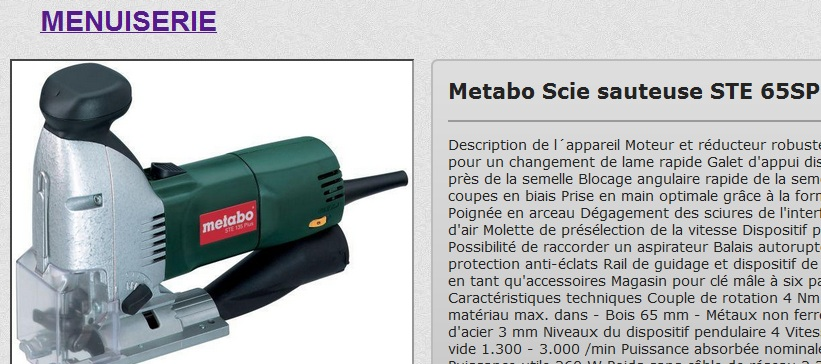
\includegraphics[scale=0.5]{Images/demofichepro.jpg}\\

\item Donner des informations sur la société et sur le service client, ainsi que sur les administrateurs du site.
Le client veut savoir à qui il a affaire et sera plus enclin à acheter si il sait qu'il peut contacter quelqu'un ensuite.
Le client sera mis en confiance, ce qui est vraiment important lorsque son argent est en jeu.\\
Ces informations seront donc accessibles depuis n'importe quelle page du site grâce au menu :\\

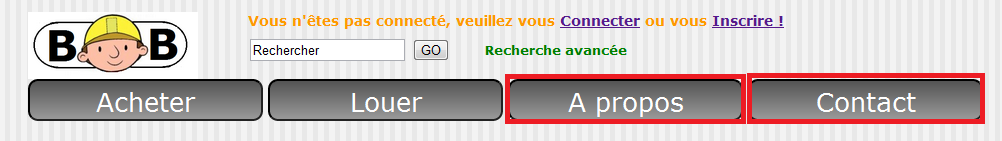
\includegraphics[scale=0.5]{Images/menu.jpg}\\

\item Ne pas trop s'introduire dans la vie privée du client : nous n'avons demandé au client que des informations non personnelles lors de son inscription : son pseudo et un mot de passe.
Il n'a pas besoin de donner son nom ni son adresse tant qu'il ne valide pas une commande.
Cela lui permettra de ne pas se sentir "tracké" et de visiter librement le site.\\

\item Un moteur de recherche bien réalisé. 
Si le client sait exactement ce qu'il veut lorsqu'il va sur le site, il ira chercher le nom du produit qu'il a en tête dans la barre de recherche.
Si le moteur de recherche n'est pas bien conçu, il risque de penser que nous n'avons pas le produit qu'il cherche et il ira donc voir ailleurs.
Si il n'a qu'une idée très vague, il y a alors des chances qu'il se tourne vers le moteur de recherche avancée.
Cela nous permettra de cerner ses critères de prix par exemple.\\

\item Mettre en évidence le produit en mettant une image assez grande : trop de site proposent encore des images ridiculement petites, ce qui peut décourager le client d'acheter, car il ne peut pas bien voir le produit et peut même penser qu'il y a des risques de "tromperie" sur la marchandise.\\

\item Une navigation aisée, c'est-à-dire des catégories bien organisées. Bien que notre site permette d'afficher à la fois des produits et des catégories sur une même page, cela sera à éviter dans le cas général. Enfin, il faudra veiller à ne pas créer de catégories vides, ce qui prendrait de la place pour rien et serait une source de frustration pour le client (quoi de plus désagréable que de trouver une catégorie qui correspond parfaitement à ce que l'on recherche et se rendre compte qu'elle est vide)\\

\item Mettre l'accent sur les produits : le but d'un site de e-commerce est de vendre, et nous avons donc fait attention de mettre l'accent sur les produits.
Le design est assez sobre, et les autres éléments du site n'empiètent pas sur les produits. Il y a également sur la page d'accueil des "coups-de-cœur" permettant de stimuler un achat imprévu chez le client.

\end{itemize}